
%\subsubsection{ECal Trigger overview}

The trigger system is designed to efficiently select e$^{+}$e$^{-}$ and $\mu^{+}\mu^{-}$ events by 
using information from the ECal and Muon System. For e$^{+}$e$^{-}$ events, the trigger looks for time coincidences of clusters in the top and bottom half of the ECal. The clusters also have to satisfy loose topological selections optimized on A$^{\prime}$ events to further reduce the rate. For $\mu^{+}\mu^{-}$ events, signals from at least the first two layers of the muon hodoscopes are combined with an ECal signal consistent with a minimum ionizing particle (MIP). 

As described above in Sec.~\ref{sec:fadc_daq}, the first stage of the trigger logic is incorporated into the FPGA's on the FADC boards which sends crystal energy and time information to the CTP. With the available 3-bit time information, the CTP can in principle look for time coincidence of crystal signals with 4~ns resolution (HPS will use a 8~ns time coincidence interval). The final trigger decision is made in the CTP and Sub-System Processor (SSP). The Trigger Supervisor generates all necessary signals and controls the entire DAQ system readout through the Trigger Interface (TI) units. The TI units are installed in every crate that participate in the readout process. 

The trigger system is free-running and driven by the 250~MHz global clock and has essentially zero dead time at occupancies expected by HPS. The Trigger Supervisor can apply dead time if necessary, for example on a 'busy' or 'full' condition from front-end electronics. The system is designed to handle trigger rates above 50~kHz and a latency set to $\approx 3~\mu$s to match that required by the SVT APV25 chip. 


 


% The proposed trigger system is nearly deadtimeless. 
%The trigger logic will search for a time coincidence between two clusters in opposite halves of the ECal for ($e^+e^-$) trigger and two MIP signatures in opposite halves of ECal and at least in the first 2 layers of the muon hodoscopes for ($\mu^+\mu^-$) trigger. The coincidence time window is programmable with 4ns resolution. The maximum trigger decision time (latency) is currently set to 3 $\mu$s for Level 1. That value is defined by the SVT readout APV25 chip.


%The first stage components of the trigger logic are incorporated into FPGAs of the Flash ADC board's, while the final decision is made in a Crate Trigger Processors (CTPs) and  Sub-System Processor (SSP) . As described above, 
%FADC sends 13-bit pulse energy and time information to CTP. With available 3-bit time information, CTP can in principal look for coincidence between different channels in 4 ns time window. For the HPS L1 trigger formation, the time window for channel coincidence will be set to 8 ns.



\vspace{1cm}
{\bf $e^+e^-$ Trigger} 


The trigger system for e$^+$e$^-$ events can be broken down into three sections (see Fig.~\ref{fig:hps_trigger_cal}):
 \begin{itemize}
 \item FADC (pulse finding): Samples and digitizes the signal pulses from each detector channel. Sends the measured pulse energy and arrival time to the CTP.
\item CTP (cluster finding): Groups FADC pulses from each half of the ECal into clusters. The cluster energy, arrival time, and hit pattern are sent to the SSP.
 \item SSP (cluster pair finding): Searches for time coincidence of pairs of clusters from the top and bottom half of the ECal and applies topological selections.
\end{itemize}
 \begin{figure}[t]
 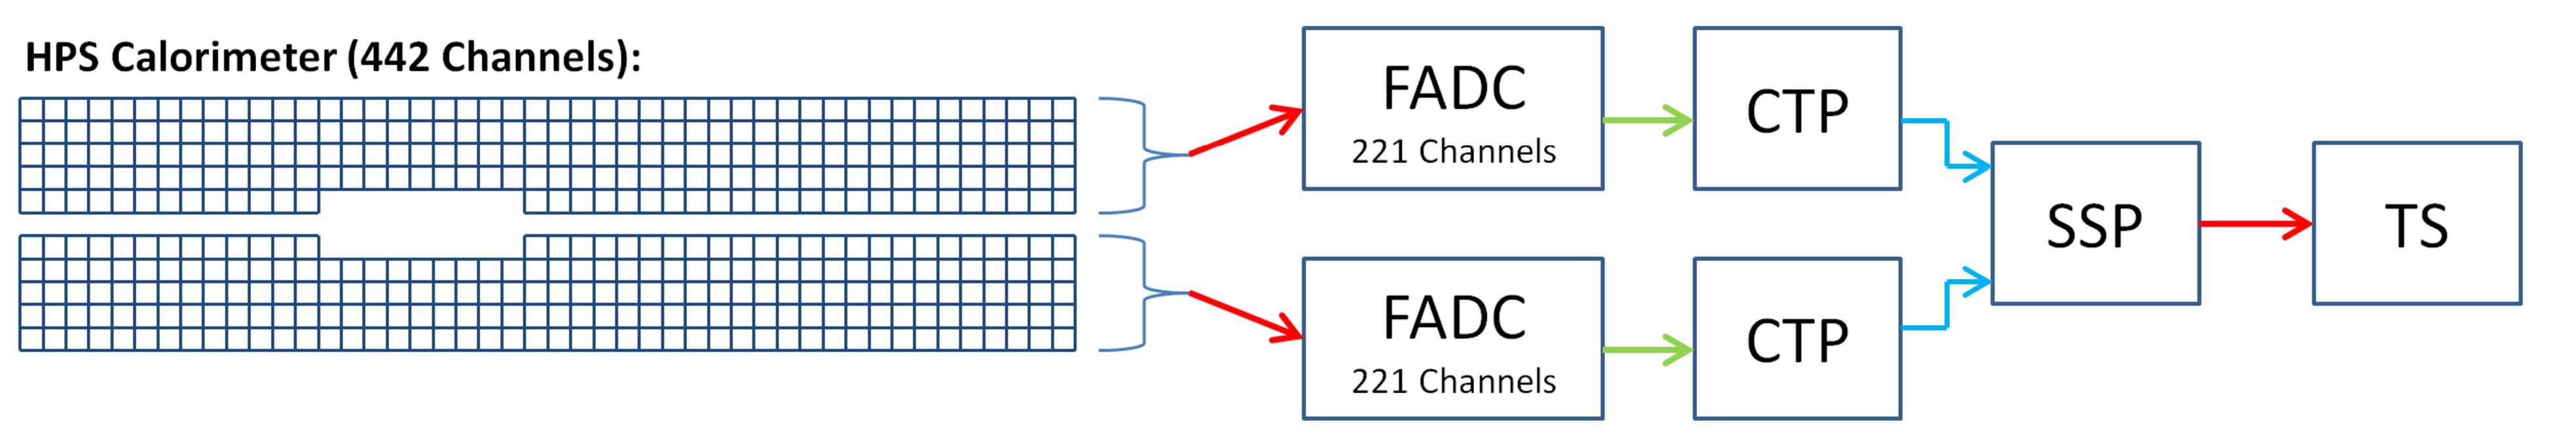
\includegraphics[scale=0.25]{daq_trigger/figures/hps_trigger_cal}
\caption{\small{Block diagram of the ECAL trigger system consisting of the FADC that samples and digitizes the detector channel signals and sends them for cluster finding in the CTP. The CTP clusters are sent to the SSP where the final trigger decision is taken based on pairs of clusters in both halves of the ECal. The decision is sent to the Trigger Supervisor (TS) that generates the necessary signals to readout the sub-detectors.}}
 \label{fig:hps_trigger_cal}
 \end{figure}
The time coincidence window of pairs of clusters in the top and bottom half of the ECal are programmable with 4~ns resolution. 
%The trigger system to look for  e$^+$e$^-$ events can be broken down into the three sections (see Fig.~ref{fig:hps_trigger_cal}):
% \begin{itemize}
 %\item FADC (pulse finding): Samples the detector channel to find pulses above the preset trigger threshold. Pulse energy and times are sent to CTP
% \item CTP (cluster finding): Searches FADC pulses (from half of calorimeter) to find clusters. Cluster energy, time, and hit pattern sent to SSP
% \item SSP (cluster pair finding): Searches CTP clusters (from top and bottom) to find cluster pairs and creates the trigger. Trigger cuts on pairs decide final trigger.
% \end{itemize}
The cluster finding algorithm is very fast and makes use of the parallel processing nature of FPGA's by simultaneously searching for 125 clusters, up to 3x3 in size, across the calorimeter crystal array, see 
Fig.~\ref{fig:hps_trigger_3x3}. 
\begin{figure}[h]

\includegraphics[scale=0.4]{daq_trigger/figures/hps_trigger_3x3}
\caption{\small{Cluster finding algorithm.}}
\label{fig:hps_trigger_3x3}
\end{figure}
It performs the following tasks:
\begin{itemize}
\item Adds energy from hits together for every 3x3 square of channels in ECal.
\item Hits are added together if they occur (leading edge) within a programmable number of 4~ns clock cycles of each other (HPS will use 8~ns time coincidence time interval).
\item If the 3x3 energy sum is larger than the programmable cluster energy threshold and the sum is greater than any neighboring 3x3 windows, the CTP reports the cluster parameters (time, energy, position and 3x3 hit pattern) to the SSP. 
\end{itemize}
The CTP evaluates all hits in its half of the calorimeter every 4~ns. A programmable time window is used to allow hits that are out of time with each other to be considered as part of a cluster sum. This is done by reporting hits when they occur and then reporting them again for the next $N$ number of 4~ns clock cycles, where $N \in [0,7]$. This is useful to deal with skew and jitter that develop from the detector, cabling, and electronics. As described above, the CTP only selects the 3x3 window with the highest energy sum of its neighbors. This filtering is applied to deal with overlapping clusters and cases where the cluster is larger than a 3x3 window.
%A 3x3 window with an energy sum above threshold and a time stamp within a programmable time window the cluster processor will report this cluster to the SSP only if the energy is greater than energies of all neighboring (up, down, left, right, and diagonals) 3x3 window clusters for that clock cycle. If the energy is not greater than its neighbor it will not be reported, instead the neighbor with larges energy will be reported. The reason for this filtering is because there are several 3x3 windows that overlap and see the sample crystals and also many clusters are larger than a 3x3 window.


The CTP sends the following information about the clusters to the SSP:
\begin{itemize}
\item 13-bit cluster energy (MeV).
\item Cluster position (crystal index: x,y).
\item Cluster time (with 4~ns resolution).
\item Cluster 3x3 hit pattern (the detector channels reporting a hit in the cluster).
\end{itemize}
The cluster position is the coordinate of the peak crystal energy as seen from a 3x3 view. The 3x3 cluster hit pattern can be used by the SSP to help filter strange cluster patterns and/or make a low resolution cluster centroid computation.
%{\bf Sub-System Processor} 
%The cluster's time, energy, position and 3x3 pattern found in two VXS crates are reported to the Sub-System Processor. 
The SSP collects the cluster information from the two halves of the calorimeter and further applies topological selections optimized to further reduce background rates with small impact on the e$^{+}$e$^{-}$ signal:
\begin{itemize}
\item Energy sum,  
$E_{min}\le E_{top}+E_{bottom}\le E_{max}$
\item Pair time coincidence, 
$|t_{top}-t_{bottom}|\le \Delta t_{max}$ 
\item Energy difference, 
$|E_{top}-E_{bottom}|\le \Delta E_{max}$ 
\item Energy slope,
$E_{cluster\_with\_min\_energy}+R_{cluster\_with\_min\_energy}\times F_{energy}\le Threshold_{slope}$
\item Co-planarity, 
$|
tan^{-1}(\frac{X_{top}}{Y_{top}})-
tan^{-1}(\frac{X_{bottom}}{Y_{bottom}}) |\le Coplanarity_{angle}$
\item Number of hits in 3x3 window, 
\#$hits_{3\times 3}\ge HitThreshold$
\end{itemize}
\noindent
where $ E_{max}$,  $\Delta t_{max}$, $ \Delta E_{max}$ , $Threshold_{slope}$, 
$F_{energy}$, $Coplanarity_{angle}$
and
$HitThreshold$ are programable parameters.

The SSP can also create a trigger decision based on the existence of a single cluster in the ECal exceeding the energy threshold which is  useful for commissioning and calibration runs. 

Online event analysis will be provided to be compared against trigger event data for immediate verification (on each trigger cut: cluster energies, positions, timing, energy slope, coplanarity and hit threshold). With identical trigger and data readout paths and high energy resolution, very precise agreement can be expected between trigger and readout.




\vspace{1cm}
%\subsubsection{Muon Trigger}
{\bf $\mu^+\mu^-$ Trigger} 

%The muon trigger will look for an energy deposition consistent with that of a MIP particle in single ECal channels and in the muon hodoscopes from a $\mu^+\mu^-$ pairs.  The CTPs in the three VXS crates (two for each half of the ECal and one for the Muon System) will search for MIP hits using energy selections on the hits reported by the FADCs satisfying: $E_{MIP}^{min}<E_{ECal\_channel}<E_{MIP}^{max}$ for the ECal and $E_{MIP_thr}<E_{\mu\_hodo}$ for the Muon System. The CTP in the Muon System will use time information of the reported MIP hits to select coincidences in three planes of each hodoscope layer according to the geometry of horizontal and vertical strips. After the MIP hits in the ECal and in the muon system are selected, the CTP sends the time and position information of each selected hit to the SSP. The SSP will look for time and position coincidence of MIP hits in the ECal with hits in at least the tthree first layers of the Muon System, treating the top and bottom halves of the detector separately. To form the final $\mu^+\mu^-$ trigger decision it will select pairs of MIP hits in opposite quadrants of the detector (similar to the coplanarity requirements described above) that are within a programmable coincidence time window. 

The muon trigger will look for 
$\mu^+\mu^-$ pairs by finding energy depositions consistent with those expected from minimum ionizing particles in the layers of the muon system.  
The trigger algorithm in the CTP of the muon system  VXS crate will produce a muon pair trigger in four steps:
\begin{itemize}
\item search for MIP hits using energy selections on the hits reported by the FADCs which satisfy $E_{MIP}^{thr}<E_{\mu\_hodo}$
\item use the time information of the reported MIP hits to select coincidences between the two planes of each hodoscope layer, quadrant by quadrant.  
\item look for coincidences in successive quadrants of at least the first three layers of the muon hodoscopes 
\item select pairs of triple coincidences in opposite quadrants of the detector and report the times and positions of coincident triple hits 
to the SSP 
\end{itemize}
If it is necessary to reduce the rate further, the SSP can in addition look for time and position coincidences of MIP hits in the ECal, defined in the ECal 
crate CTPs as hits with 1 or 2 crystals and energy within predefined thresholds: $E_{MIP}^{min}<E_{ECal\_channel}<E_{MIP}^{max}$. 
The SSP will send the final decision regarding the $\mu^+\mu^-$ trigger to the Trigger Supervisor  board. 


\vspace{1cm}
{\bf Diagnostic Tools}

The previous experience with the similar (but much simpler) trigger system showed that diagnostic tools are necessary to make sure that the calorimeter and trigger electronics work as expected. 

Scalers will be implemented for every ECal channel. The example of this diagnostic tool is presented in Fig.~\ref{fig:dvcs_beam}
from the previous version of the calorimeter. Hot or dead channels are easily identified and disabled online.
\begin{figure}[h]
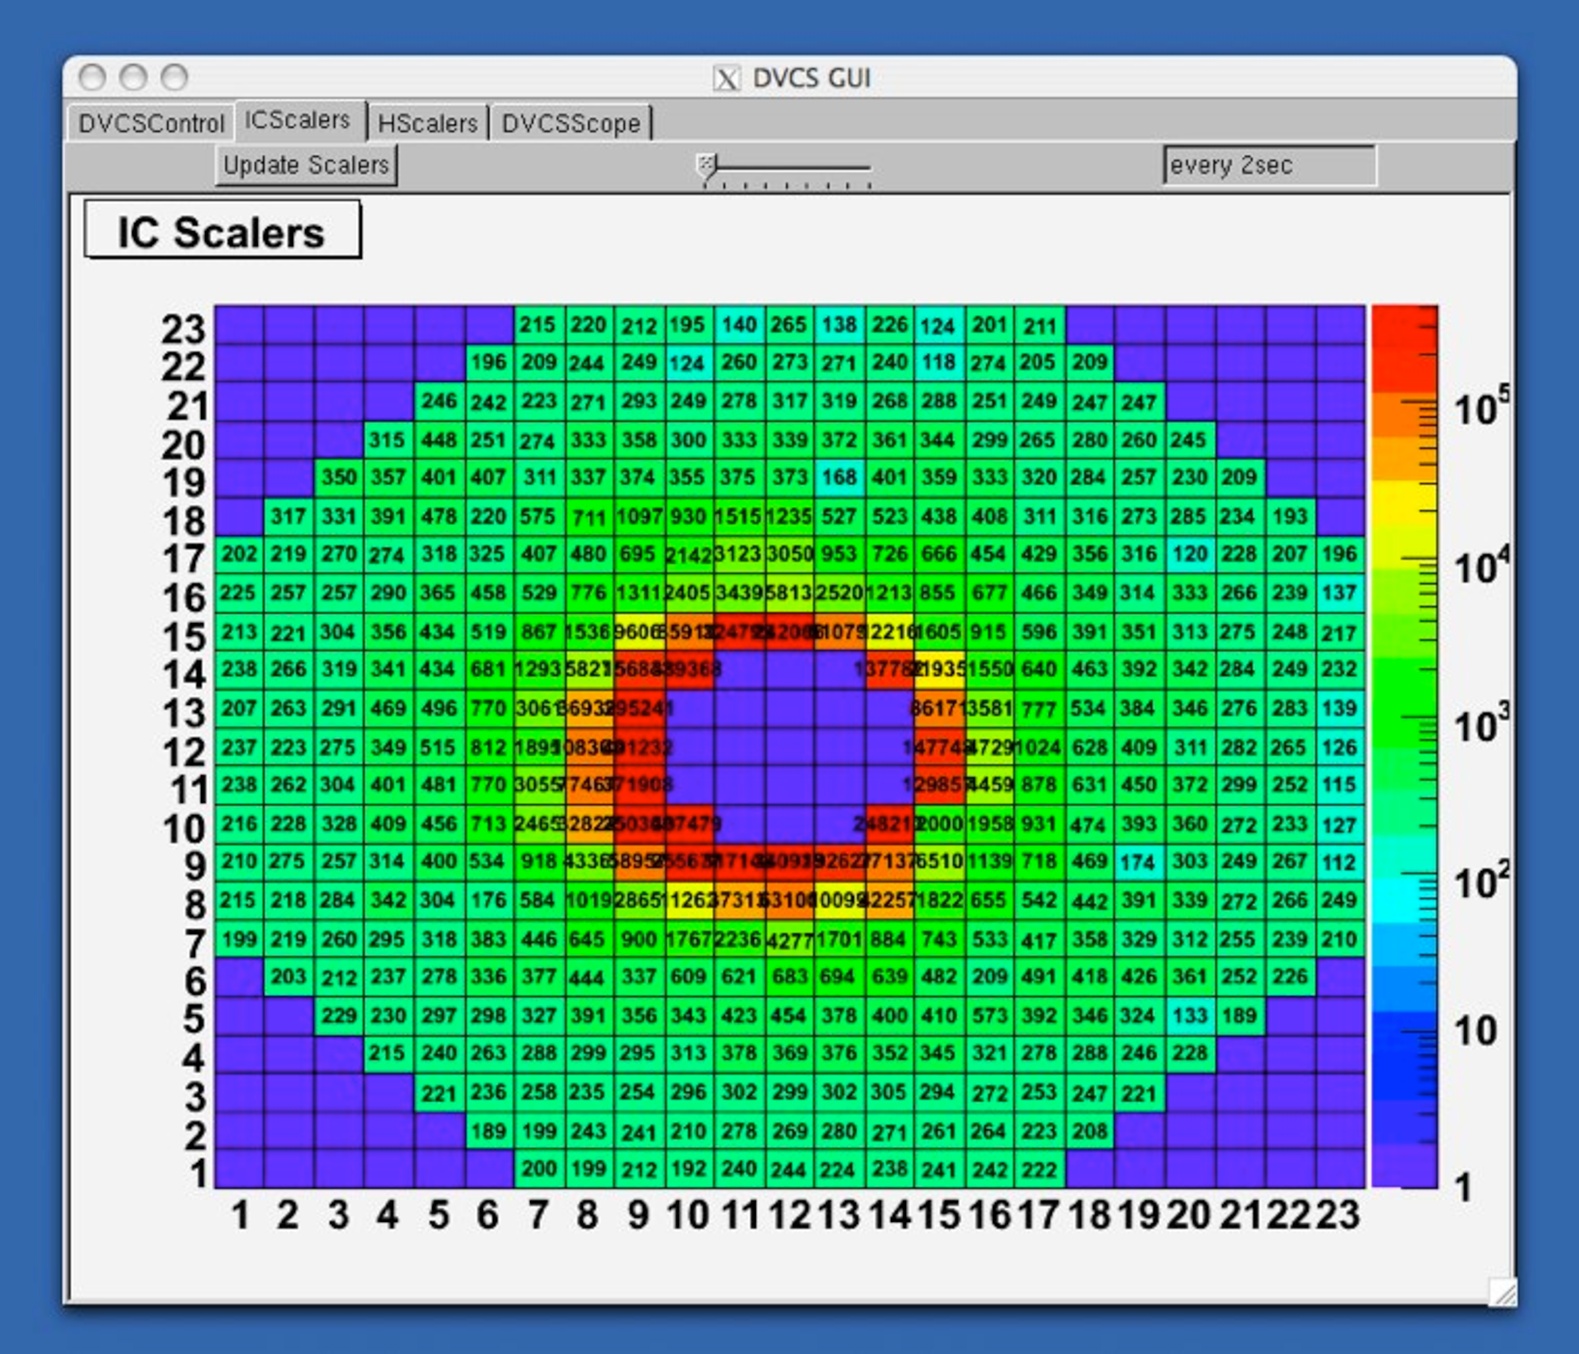
\includegraphics[scale=0.52]{daq_trigger/figures/dvcs_beam}
\caption{\small{Scalers (example from the previous version of the calorimeter).}}
\label{fig:dvcs_beam}
\end{figure}
Diagnostic scope permits to analyze on-line  the trigger logic. The goal to have  the Two-Dimensional Analyzer
 is to provide a remote debug interface to identify bad channels, verify cluster finding algorithms and check timing.
 The details of this analyzer are as following:
 
\begin{itemize}
\item Logic analyzer runs in parallel, non-intrusive, to the calorimeter trigger
\item Can setup trigger on any ECal pixel arrangement and/or cluster count
\item Can move forward/backward in time by ~250 ns to see timing details
\item Will be customized for HPS geometry and hardware
\end{itemize}

The example of the 2D analyzer is presented in Fig.~\ref{fig:dvcs_2_cluster}. Two clusters are displayed
in the picture. The red color displays the hits in the calorimeter and  the center of clusters is displayed in yellow.

In addition to the scalers, the distributions on individual ADC channel pulse energy will be provided.
The cluster hits positions and energy from SSP processor will be histogrammed as well. Two histograms (accepted and rejected) will be provided for each trigger cut used in the trigger logic.



\begin{figure}[t]
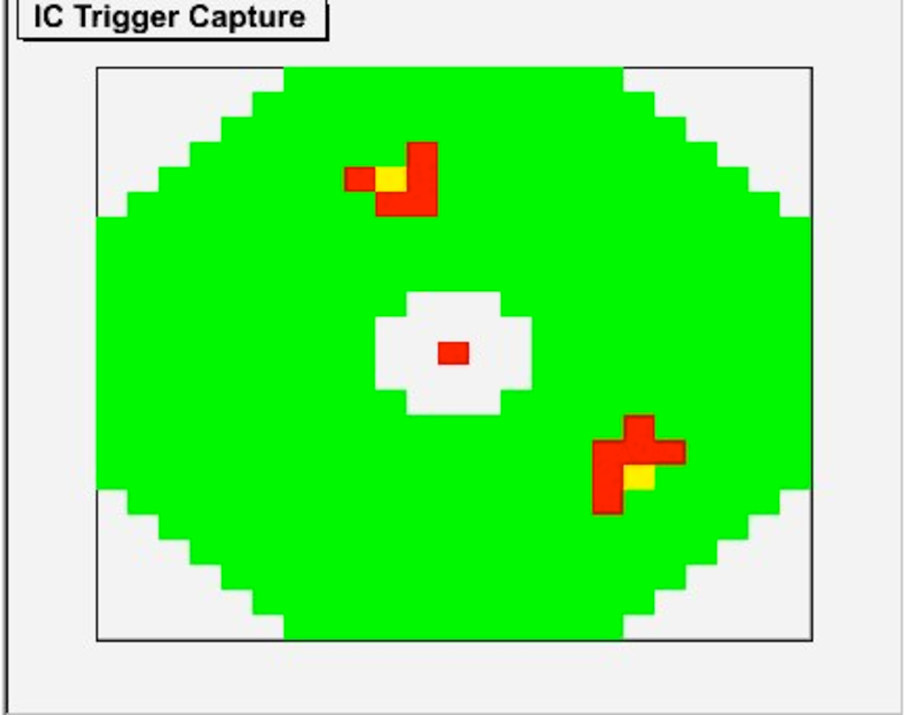
\includegraphics[scale=0.8]{daq_trigger/figures/dvcs_2_cluster}
\caption{\small{Diagnostic scope (example with two clusters found from the previous version of the calorimeter). Green - no hits, red - tower with hit, yellow - cluster found.}}
\label{fig:dvcs_2_cluster}
\end{figure}




